% !TEX root = ../lab2_report.tex
% ═══════════════════════════════════════════════════════════════
% 实验五：平面叶栅攻角特性测量
% ═══════════════════════════════════════════════════════════════

\section{实验五：平面叶栅攻角特性测量}

\subsection{实验目的}

\begin{enumerate}
    \item 认识叶栅流动损失以及气流转折角的攻角特性。
    \item 了解三孔探针测量原理及坐标架操作方法。
    \item 掌握气动参数的测量方法及数据处理方法。
    \item 理解叶栅攻角特性与额定特性的联系。
\end{enumerate}

\subsection{实验原理}

叶栅在一定进口马赫数下的气动性能主要受来流攻角影响。攻角改变时，叶片表面附面层的发展和分离位置随之变化，从而影响气流转折能力（转折角 $\Delta\beta$）和流动损失（总压损失系数 $\omega$）。在额定攻角（设计攻角）附近，损失最小、转折角适中，偏离额定攻角后损失急剧增大。通过三孔探针测量叶栅出口中间截面的气流参数，可获得叶栅的攻角特性曲线。

\subsection{实验装置}

\subsubsection{叶栅风洞}

使用与实验四相同的平面叶栅风洞和 NACA-65 叶型叶栅（参数同实验四表~\ref{tab:cascade_params}）。

\subsubsection{三孔气动探针与位移机构}

三孔探针安装在三自由度位移机构上，可沿轴向（导轨1）、周向（导轨2）和径向移动，并可通过转台绕自身轴线旋转。三孔探针的工作模式为"对向测量"：旋转探针转台使左右孔（孔1、孔3）压力相等时，中间孔（孔2）正对来流方向，孔2读数即为当地总压 $P_2^*$，转台刻度指示当地气流角 $\beta_2$。出口静压 $P_2$ 由壁面静压孔或探针静压孔获取。

\subsection{实验步骤}

\begin{enumerate}
    \item 记录实验室大气温度和压力，明确实验分工。
    \item 启动离心风机，等待流动稳定。
    \item 水排稳定后，记录叶栅进口总压 $P_1^*$ 和静压 $P_1$。
    \item 将三孔探针移至适当位置（导轨1示数=5 cm，对准第3-4号叶片中间流道）。
    \item 转动探针转台，使三孔探针孔1、孔3压力相等（对向测量）。
    \item 记录出口总压 $P_2^*$、静压 $P_2$、探针转盘刻度 $\beta$（即出口气流角 $\beta_2$）。
    \item 沿栅距方向（导轨2）移动探针，在4个等间距位置重复步骤\textbf{5-6}，取算术平均值以消除周向不均匀性。
    \item 改变叶栅转盘角度以改变攻角（$-15\textdegree$、$-10\textdegree$、$-5\textdegree$、$0\textdegree$、$+5\textdegree$、$+7\textdegree$），重复步骤\textbf{3-7}。
    \item 实验结束：关闭风机，整理设备。
\end{enumerate}

\subsection{数据处理方法}

\subsubsection{进口气流角和攻角}

\begin{equation}
    \beta_1 = 25\textdegree + \gamma, \quad i = \beta_1 - 35.6\textdegree
\end{equation}

\subsubsection{气流转折角}

\begin{equation}
    \Delta\beta = \beta_2 - \beta_1
\end{equation}

$\Delta\beta$ 表示气流经过叶栅通道后方向改变的角度，反映叶栅的导流和加功能力。

\subsubsection{总压损失系数}

\begin{equation}
    \omega = \frac{P_1^* - P_2^*}{P_1^* - P_1}
\end{equation}

$\omega$ 表征叶栅的流动损失：分子为总压损失，分母为进口动压。$\omega$ 越大表示损失越严重。

\subsection{数据处理结果及分析}

\subsubsection{攻角特性曲线}

\begin{figure}[H]
    \centering
    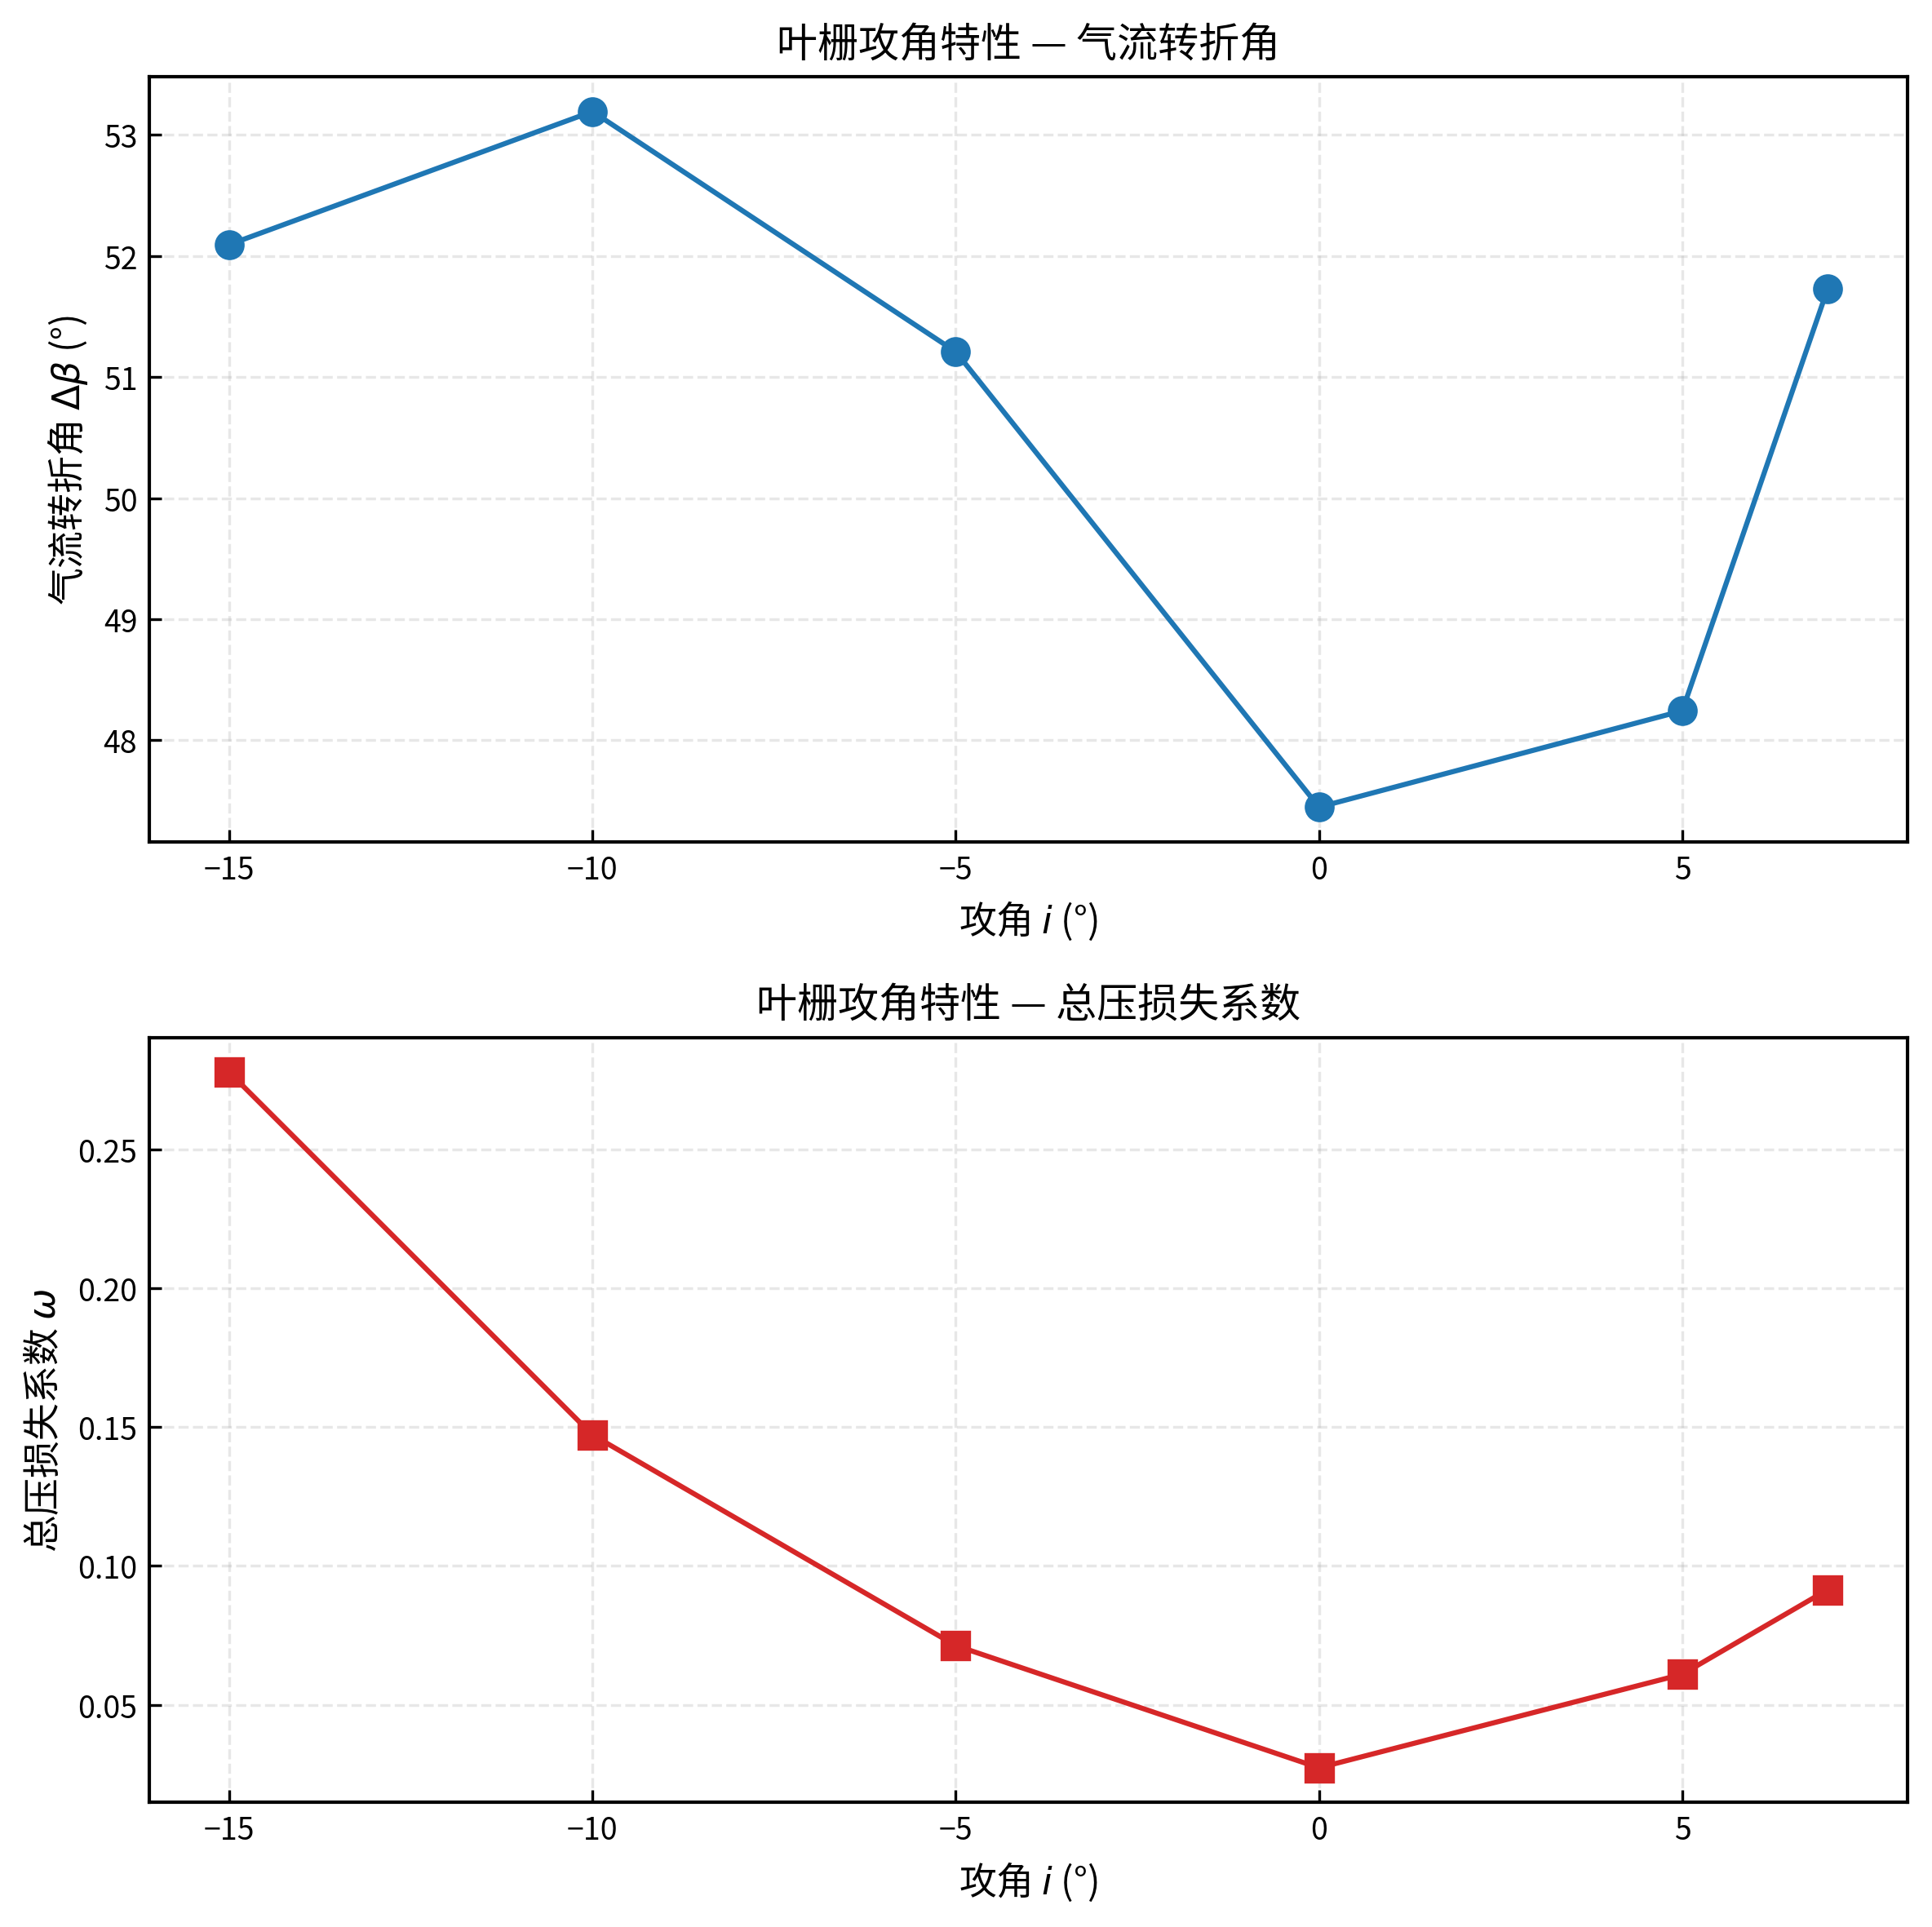
\includegraphics[width=0.85\textwidth]{figures/exp5_attack_angle_characteristics.png}
    \caption{叶栅攻角特性曲线（转折角 $\Delta\beta$ 与损失系数 $\omega$）}
    \label{fig:attack}
\end{figure}

图~\ref{fig:attack} 展示了 $-15\textdegree$ 至 $+7\textdegree$ 攻角范围内的转折角和损失系数变化。

\subsubsection{结果分析}

\begin{enumerate}
    \item \textbf{转折角 $\Delta\beta$ 的攻角特性}：
    \begin{itemize}
        \item $\Delta\beta$ 在 $-15\textdegree \sim +5\textdegree$ 范围内随攻角近似线性增大，斜率约为 0.3\textdegree/\textdegree。
        \item 在 $+5\textdegree$ 以上，$\Delta\beta$ 的增长率减小，曲线趋于平缓甚至下降，反映叶片的气流转折能力接近极限——吸力面附面层开始大范围分离，有效流通面积减小。
    \end{itemize}
    \item \textbf{损失系数 $\omega$ 的攻角特性}：
    \begin{itemize}
        \item $\omega$ 在设计攻角（$0\textdegree$）附近取得最小值，呈典型的"抛物线"形或"浴盆"形曲线。
        \item 偏离设计攻角后 $\omega$ 急剧增大。$-15\textdegree$ 时负攻角过大，压力面可能出现分离；$+7\textdegree$ 时正攻角过大，吸力面出现大面积分离。
        \item 正攻角侧的损失增长比负攻角侧更剧烈，因为吸力面逆压梯度增大导致的附面层分离比压力面更严重。
    \end{itemize}
    \item \textbf{与额定特性的联系}：
    \begin{itemize}
        \item 压气机的额定工作点（设计点）对应损失最小、效率最高的攻角范围。
        \item 偏离额定状态时，损失增大、效率下降、增压能力降低，反映了叶栅攻角特性向压气机整机特性的传递关系。
    \end{itemize}
\end{enumerate}

\subsection{结论}

成功测量了NACA-65叶栅在 $-15\textdegree$ 至 $+7\textdegree$ 攻角范围内的气流转折角 $\Delta\beta$ 和总压损失系数 $\omega$ 的攻角特性。$\Delta\beta$ 随攻角近似线性增大但在大正攻角时趋于饱和；$\omega$ 在 $0\textdegree$ 攻角附近最小，偏离后急剧增大，符合典型压气机叶栅攻角特性的基本规律。实验结果与《航空叶片机原理》中关于叶栅额定特性的理论分析一致。
